\documentclass[a4paper, 11pt]{article}
%\documentclass{article}
\usepackage[utf8]{inputenc}
\usepackage{hyperref}
\usepackage{calc}
%\usepackage{fourier} %% changes everything to sans-serif!
\usepackage{amssymb}
\usepackage{amsmath}
\usepackage{amsthm}
\usepackage{amsfonts}
\usepackage{mathtools}
\usepackage{textcomp}
%\usepackage{tikz}
\usepackage{tikz-cd}
\usetikzlibrary{cd}
\usepackage{dirtytalk}
\usepackage{titlesec}
\usepackage{verbatim}
\usepackage{pdfpages}
\usepackage{caption}
%%\captionsetup[figure]{labelfont=footnotesize}
\usepackage{hyperref}
\usepackage{parskip}

%% neu
\usepackage{physics}
\usepackage{accents} %% for multiple subscripts
\usepackage{fancyhdr} %% for header and footer
\usepackage[a4paper, left=2.5cm, right=2.5cm, top=2cm]{geometry}
\usepackage{graphicx} % Required for inserting images
%\usepackage[ngerman]{babel}
\usepackage{csquotes}
\MakeOuterQuote{"}

\title{Building a pan flute}
\author{Catharina Hock, Stefanie Hövermann}
\date{August  2026}

\newcommand{\answerline}[1][0.5cm]{%
    \noindent\rule{#1}{0.4pt}
}

\begin{document}
\maketitle 

\section{Theoretical part}
Now, we're going to put our understanding of acoustics to the test to build our very own instrument; a pan flute! 

\begin{figure}[!htb]
    \centering
    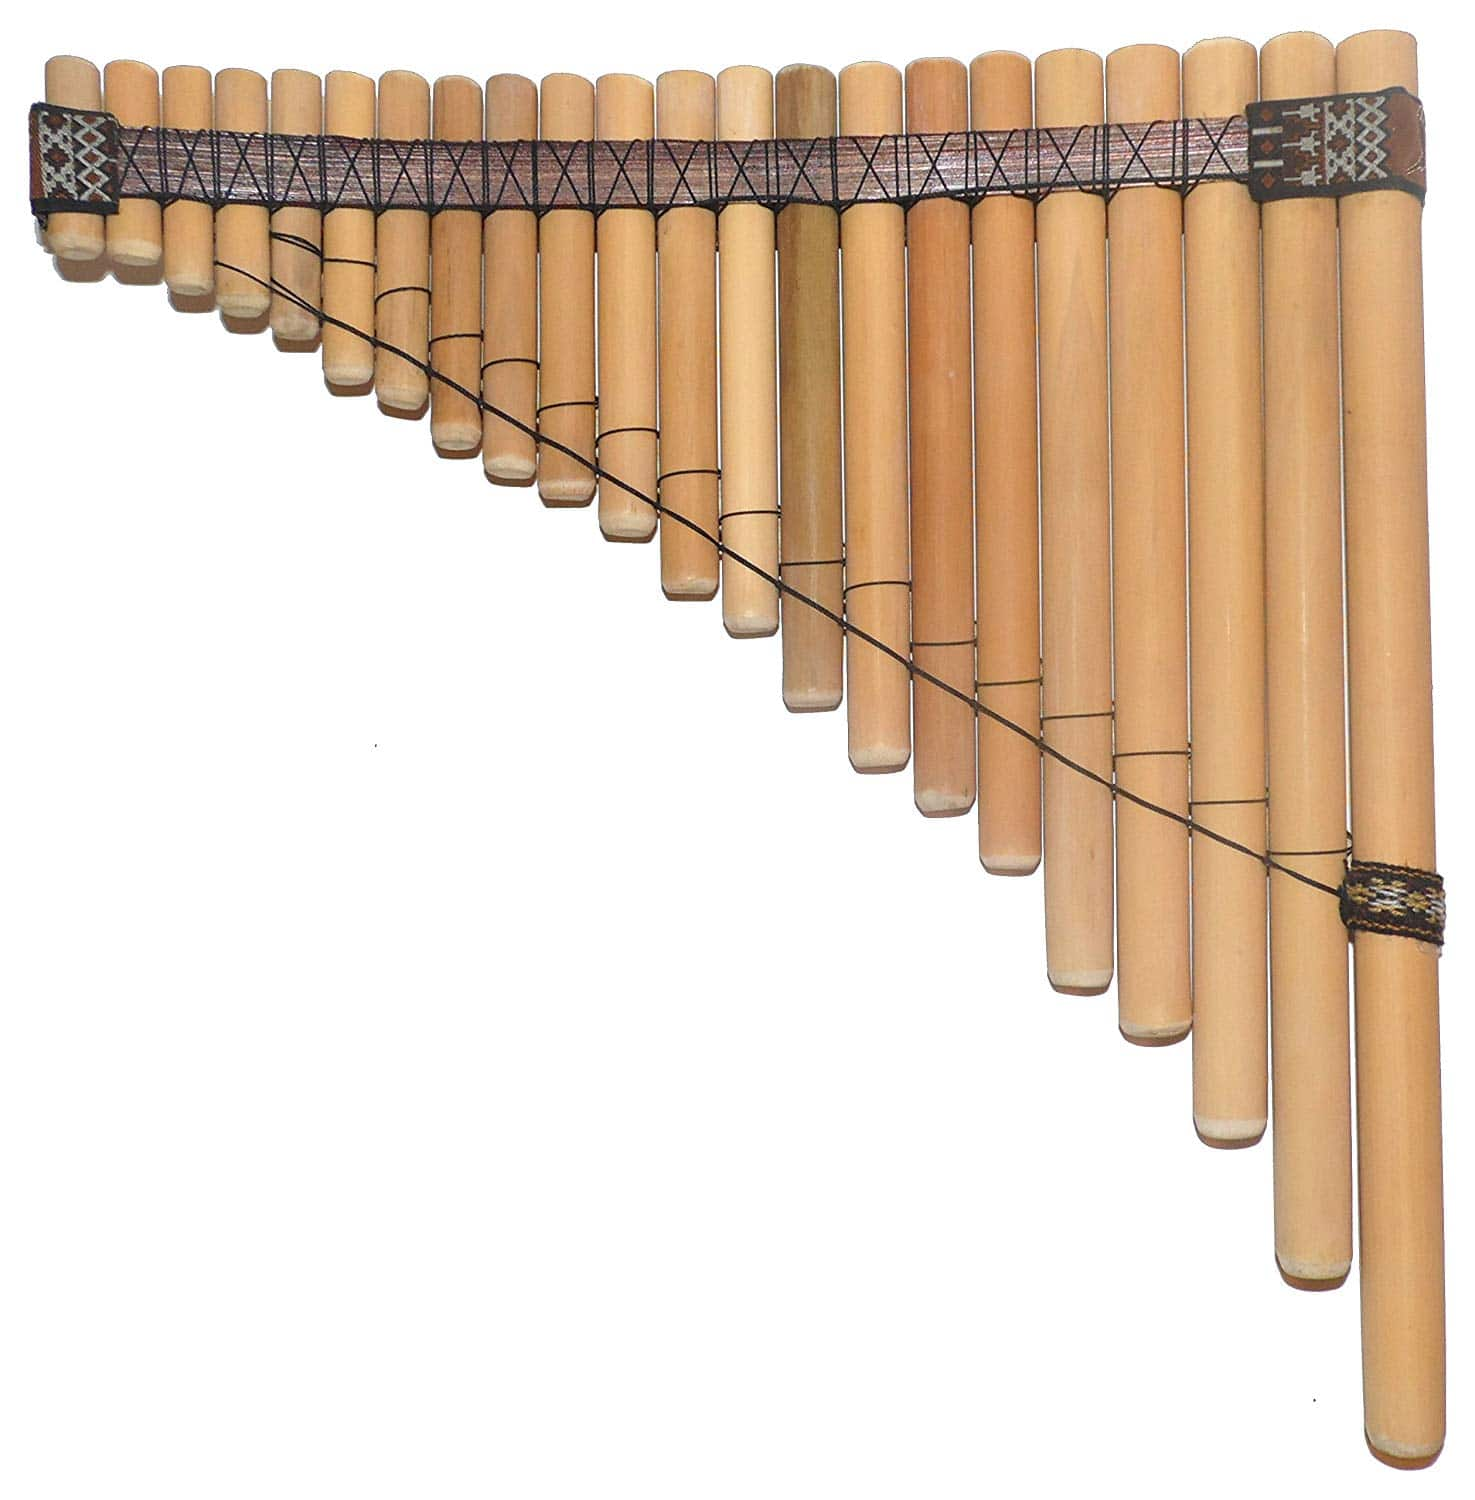
\includegraphics[width = 0.6 \textwidth]{Bilder/pan_flute.jpg}
    %Quelle : https://primesound.org/wp-content/uploads/2019/12/Peru-Treasure-Pan-Flute-Antara-3.jpg
    \caption{A pan flute. }
    \label{fig:pan}

\end{figure}

As can be seen in Fig. \ref{fig:pan}, a pan flute consists of many individual pipes. Each pipe will produce a specific tone when you blow over it. 

\textit{Question: Try to explain in your own words why this works. What happens if you blow over a pipe?}

\textit{Question: Have a closer look at Fig. \ref{fig:pan}. Do you notice something interesting about the lengths of the pipes? Do they get longer linearly? Logarithmically? Exponentially? Do you have an idea why? Remember what we learned about tuning systems.}

After learning about different tuning systems, we know which frequencies we need to include to be able to play in a certain key. 
Before we get into this, recall that in our discussion of waves, we talked about harmonic waves in pipes with one and two fixed ends. Recall that the conditions for the occurring wavelengths were 

\begin{align}
    l = n \cdot \frac{\lambda}{2}
\end{align}

for the n-th mode in a medium with two fixed ends, and 

\begin{align}
    l = (2n+1) \cdot \frac{\lambda}{4}
\end{align}
For the n-th mode for a medium with one fixed and one free end.

How does this translate to the case of the pipes? Having two closed off ends for a pipe seems very impractical, because there's no way to blow over it and excite an oscillation. In fact, we must think carefully about what fixed and free ends even mean in the context of sound, which are pressure waves.

\textit{Question: At the open end of the pipe, can air flow in and out? Can the pressure change? What about the closed end? Can the air flow in and out? Can the pressure change? How does this correspond to free and fixed ends?}

\textbf{Answer:} Thinking about this carefully, we see that at the \textbf{open} end of the pipe, the pressure is \textbf{fixed}, since it must always be equal to the pressure outside of the pipe, which is just the atmospheric pressure. On the other hand, the air can move in and out freely through the open end. 
At the \textbf{closed} end of the pipe, the pressure is \textbf{free} to take pretty much any value, whereas the air cannot flow through it.

This means that a pipe with two open ends corresponds to the case of a medium with two fixed ends, because the pressure will be fixed at both ends!

\textit{Question: Assuming we want our lowest note to be as low as possible, with a finite amount of pipes available to us, which should we choose? Pipes with two open ends or pipes with one open and one closed end? Why?}

\textbf{Answer:} The lower the pitch of the note, the lower the frequency will be, and hence the larger the wavelength will be. So we want to maximize the wavelength of the first mode of a given pipe of length $l$. If we leave both ends open, the first harmonic will have $l=\lambda/2$, so $\lambda = 2l$. If we close one end, the first mode will satisfy $l = \lambda/4$, so $\lambda = 4l$, which is clearly bigger. Hence, we should use pipes with one closed and one open end.

With this settled, we can finally begin our calculations. We'll only use this formula from now on:
\begin{align}
    \lambda = 4 l 
\end{align}
which gives the first harmonic of a pipe with one closed and one open end which has length $l$. 

\textit{Question: What is the frequency of this first harmonic?}

\textbf{Answer:} Recall $v \approx 340$ m/s at $20^\circ$C. Furthermore,
\begin{align}
    v = \lambda \cdot f 
\end{align} 
Rewriting this, we obtain
\begin{align}
    f = v/\lambda = \frac{v}{4l}.
\end{align}

\textit{Question: How long would the pipe have to be to produce the middle A, so $f = 440$ Hz? What about a pipe with two open ends?}

\textbf{Answer:} We rewrite the previous equation
\begin{align}
    l = \frac{v}{4f}
\end{align}
So $l = 19.3$ cm. This is a bit unwieldy, but still much better than the $38.6$ cm we would have needed for a pipe with two open ends!

\textit{Question: Using equal temperament, calculate the pipe lengths for the chromatic scale.}

\textbf{Answer:}

\begin{table}[ht]
    \centering
    \begin{tabular}{cc|cc|cc}
        \textbf{Note} & \textbf{Length (cm)} &
        \textbf{Note} & \textbf{Length (cm)} &
        \textbf{Note} & \textbf{Length (cm)} \\ \hline
        $A_4$        & 19.3 & $A_5$        & 9.7 & $A_6$        & 4.8 \\
        $A^\sharp_4$ & 18.2 & $A^\sharp_5$ & 9.1 & $A^\sharp_6$ & 4.6 \\
        $B_4$        & 17.2 & $B_5$        & 8.6 & $B_6$        & 4.3 \\
        $C_5$        & 16.2 & $C_6$        & 8.1 & $C_7$        & 4.1 \\
        $C^\sharp_5$ & 15.3 & $C^\sharp_6$ & 7.7 & $C^\sharp_7$ & 3.8 \\
        $D_5$        & 14.5 & $D_6$        & 7.2 & $D_7$        & 3.6 \\
        $D^\sharp_5$ & 13.7 & $D^\sharp_6$ & 6.8 & $D^\sharp_7$ & 3.4 \\
        $E_5$        & 12.9 & $E_6$        & 6.4 & $E_7$        & 3.2 \\
        $F_5$        & 12.2 & $F_6$        & 6.1 & $F_7$        & 3.0 \\
        $F^\sharp_5$ & 11.5 & $F^\sharp_6$ & 5.7 & $F^\sharp_7$ & 2.9 \\
        $G_5$        & 10.8 & $G_6$        & 5.4 & $G_7$        & 2.7 \\
        $G^\sharp_5$ & 10.2 & $G^\sharp_6$ & 5.1 & $G^\sharp_7$ & 2.6 \\
    \end{tabular}
    \caption{Pipe lengths corresponding to different notes.}
    \label{tab:pipe_lengths}
\end{table}

\textit{Optional: If you prefer, you can also do this for Just tuning or Pythagorean tuning. You'll have to pick the key you want to play in first. I suggest you use the lowest note as the key the scale is in. Have a look at Tab. \ref{tab:pipe_lengths} and chose a note that has a reasonable pipe length. Then do the calculations based on that length.}

To save material, we'll only build one octave and only the diatonic scale. (So only 8 pipes in total). Pick a key to play in and choose the corresponding notes and pipe lengths from Tab. \ref{tab:pipe_lengths}.
Now that we've calculated the pipe lengths, we're all set to actually go ahead and build the pipes! 

\section{Experimental part}
If at any point you're unsure about the instructions, feel free to ask the course leaders. Be careful around the saws and the hot glue.
\begin{itemize}
    \item Make sure you have all the material you'll need. You need: a pipe (you can calculate the total length from your previous considerations), a measuring stick, a hot glue gun, sanding paper, a saw, a pencil, some clay to close off the pipes, tape, your calculations. You can share the material with the other participants.
    \item Measure your calculated pipe lengths with the measuring stick and mark the lengths with the pencil
    \item Show the course leaders your measurements and reasoning. \textbf{Do this before you start sawing the pipe! If you cut incorrectly, we might not have enough pipes for everyone.}
    \item Saw the pipes apart where you marked them with the pencil.
    \item Sand the ends of the pipes with the sanding paper. Make sure there are no splinters sticking out. Those could hurt you while playing the instrument.
    \item Block one end of each pipe with the clay.
    \item Arrange the pipes from largest to smallest. Make sure the open ends of the pipes align. This will make it easier to play. When you're satisfied with your arrangement, tape the pipes together provisorically.
    \item Now, glue the pipes together with the glue gun. Be careful, its tip is very hot! Try not to get any hot glue on your hands and your clothes, and make sure to put a piece of cardboard under your flute before starting to glue. It's quite hard to get the glue off the table again.
    \item Wait for the glue to cool off. Flip the pipe, and glue it together on the other side, too.
    \item Remove the tape.
    \item Congratulations, you now have a functional pan flute!
\end{itemize}


\end{document}